%!TEX program = xelatex
%!TEX spellcheck = en_GB
\documentclass[final]{article}
% Include all project wide packages here.
%\usepackage{fullpage}
\usepackage[a4paper,margin=2.5cm,top=2cm]{geometry}
\usepackage{polyglossia}
\setmainlanguage{english}
\usepackage{csquotes}
\usepackage{graphicx}
\usepackage{pdfpages}
\usepackage{caption}
\usepackage[list=true]{subcaption}
\usepackage{float}
\usepackage{standalone}
\usepackage{import}
\usepackage{tocloft}
\usepackage{wrapfig}
\usepackage{authblk}
\usepackage{array}
\usepackage{booktabs}
\usepackage[title,titletoc]{appendix}
\usepackage{fontspec}
\usepackage{pgfplots}
\usepackage{tikz}
\usepackage{tikz-uml}
\usepackage{siunitx}
\usepackage{units}
\usepackage{amsmath}
\usepackage{mathtools}
\usepackage{unicode-math}
\usepackage{rotating}
\usepackage{titlesec}
\usepackage{titletoc}
\usepackage{blindtext}
\usepackage{color}
\usepackage{enumitem}
\usepackage{tabularx}
\usepackage{titling}
\usepackage[%
siunitx,
fulldiodes,
europeanvoltages,
europeancurrents,
europeanresistors,
americaninductors,
smartlabels]{circuitikz}

\newcommand{\matlab}{{\textsc{matlab }}}

\usetikzlibrary{calc}
\usetikzlibrary{positioning}
\usetikzlibrary{automata}
\usetikzlibrary{arrows.meta}

\tikzstyle{every state}=[fill=tu-cyan,align=center,draw=black,line width=1pt,node distance=3cm,minimum width = 1.8cm]%for FSMs casper
\tikzstyle{every initial by arrow}=[initial text={Reset}]
\newcommand{\setpathasarrows}{\tikzstyle{every path}=[auto,line width=1.5pt,line cap=round,line join=round]}

\pgfplotsset{compat=newest}
\pgfplotsset{plot coordinates/math parser=false}
\usetikzlibrary{plotmarks}
\usepgfplotslibrary{patchplots}
\newlength\figureheight
\newlength\figurewidth

\tikzset{every axis/.style={xticklabel style={align=right}}}

\usepackage[
%backend=bibtex,
backend=biber,
	texencoding=utf8,
bibencoding=utf8,
style=numeric,
citestyle=numeric,
    sortlocale=en_US,
    language=auto,
    backref=true,
    abbreviate=false,
    date=iso8601
]{biblatex}


\usepackage{listings}
\newcommand{\includecode}[4][c]{\lstinputlisting[caption=#2, escapechar=, style=#1,label=#4]{#3}}
\newcommand{\superscript}[1]{\ensuremath{^{\textrm{#1}}}}
\newcommand{\subscript}[1]{\ensuremath{_{\textrm{#1}}}}


\newcommand{\chapternumber}{\thechapter}
\renewcommand{\appendixname}{Appendix}
\renewcommand{\appendixtocname}{Appendices}
\renewcommand{\appendixpagename}{Appendices}


\setlist[enumerate]{labelsep=*, leftmargin=1.5pc}
\setlist[enumerate,1]{label=\arabic*., ref=\arabic*}
\setlist[enumerate,2]{label=\arabic*.,ref=\theenumi.\arabic*}
\setlist[enumerate,3]{label=\arabic*., ref=\theenumii.\arabic*}

\setcounter{chapter}{-1} %start chapter numbers with 0

\usepackage{xr-hyper}
\usepackage[hidelinks]{hyperref} %<--------ALTIJD ALS LAATSTE
\usepackage[nameinlink,noabbrev,capitalise]{cleveref} %<------- Clever Ref moet na hyperref
\crefname{app}{Appendix}{Appendices}
%\renewcommand{\familydefault}{\sfdefault}


\setmainfont{Myriad Pro}[Ligatures={Common,TeX}]
%\setmathfont{Asana Math}
\setmathfont{Asana-Math.otf}
\setmonofont[Scale=0.9]{Lucida Console}
\newfontfamily\headingfont{Minion Pro}[Ligatures={Common,TeX}]


%Design colors
\definecolor{accent1}{RGB}{0,100,200}
\definecolor{accent2}{RGB}{0,50,100}
\definecolor{tu-cyan}{RGB}{0,166,214}

\newcommand{\hsp}{\hspace{20pt}}
% \titleformat{\chapter}[hang]{\Huge\headingfont}{\chapternumber\hsp\textcolor{accent2}{|}\hsp}{0pt}{\Huge\headingfont}

% \titleformat{name=\chapter,numberless}[hang]{\Huge\headingfont}{\hsp\textcolor{accent2}{|}\hsp}{0pt}{\Huge\headingfont}

% \titleformat{\section}[block]{\LARGE\headingfont}{\arabic{chapter}.\arabic{section}}{0.4em}{}
% \titleformat{\subsection}[block]{\Large\headingfont}{\arabic{chapter}.\arabic{section}.\arabic{subsection}}{0.4em}{}
% \titleformat{\subsubsection}[block]{\large\headingfont}{\arabic{chapter}.\arabic{section}.\arabic{subsection}.\arabic{subsubsection}}{0.4em}{}
\renewcommand{\arraystretch}{1.2}
\renewcommand{\baselinestretch}{1.25} 

\renewcommand\cfttoctitlefont{\headingfont\Huge}
\renewcommand\cftloftitlefont{\headingfont\Huge}
\renewcommand\cftlottitlefont{\headingfont\Huge}
\setcounter{lofdepth}{2}
\setcounter{lotdepth}{2}


\setlength{\parindent}{0pt}
\setlength{\parskip}{1em}


%SIuntix settings:
%default: 0V to 10V
%custom: 0 - 10V
\sisetup{range-phrase=--}
\sisetup{range-units=single}
\DeclareSIUnit\years{years}

%For code listings
\definecolor{black}{rgb}{0,0,0}
\definecolor{browntags}{rgb}{0.65,0.1,0.1}
\definecolor{bluestrings}{rgb}{0,0,1}
\definecolor{graycomments}{rgb}{0.4,0.4,0.4}
\definecolor{redkeywords}{rgb}{1,0,0}
\definecolor{bluekeywords}{rgb}{0.13,0.13,0.8}
\definecolor{greencomments}{rgb}{0,0.5,0}
\definecolor{redstrings}{rgb}{0.9,0,0}
\definecolor{purpleidentifiers}{rgb}{0.01,0,0.01}


\lstdefinestyle{csharp}{
language=[Sharp]C,
showspaces=false,
showtabs=false,
breaklines=true,
showstringspaces=false,
breakatwhitespace=true,
escapeinside={(*@}{@*)},
columns=fullflexible,
commentstyle=\color{greencomments},
keywordstyle=\color{bluekeywords}\bfseries,
stringstyle=\color{redstrings},
identifierstyle=\color{purpleidentifiers},
basicstyle=\ttfamily\small}

\lstdefinestyle{c}{
language=C,
showspaces=false,
showtabs=false,
breaklines=true,
showstringspaces=false,
breakatwhitespace=true,
escapeinside={(*@}{@*)},
columns=fullflexible,
commentstyle=\color{greencomments},
keywordstyle=\color{bluekeywords}\bfseries,
stringstyle=\color{redstrings},
identifierstyle=\color{purpleidentifiers},
}

\lstdefinestyle{matlab}{
language=Matlab,
showspaces=false,
showtabs=false,
breaklines=true,
showstringspaces=false,
breakatwhitespace=true,
escapeinside={(*@}{@*)},
columns=fullflexible,
commentstyle=\color{greencomments},
keywordstyle=\color{bluekeywords}\bfseries,
stringstyle=\color{redstrings},
identifierstyle=\color{purpleidentifiers}
}

\lstdefinestyle{vhdl}{
language=VHDL,
showspaces=false,
showtabs=false,
breaklines=true,
showstringspaces=false,
breakatwhitespace=true,
escapeinside={(*@}{@*)},
columns=fullflexible,
commentstyle=\color{greencomments},
keywordstyle=\color{bluekeywords}\bfseries,
stringstyle=\color{redstrings},
identifierstyle=\color{purpleidentifiers}
}

\lstdefinestyle{xaml}{
language=XML,
showspaces=false,
showtabs=false,
breaklines=true,
showstringspaces=false,
breakatwhitespace=true,
escapeinside={(*@}{@*)},
columns=fullflexible,
commentstyle=\color{greencomments},
keywordstyle=\color{redkeywords},
stringstyle=\color{bluestrings},
tagstyle=\color{browntags},
morestring=[b]",
  morecomment=[s]{<?}{?>},
  morekeywords={xmlns,version,typex:AsyncRecords,x:Arguments,x:Boolean,x:Byte,x:Char,x:Class,x:ClassAttributes,x:ClassModifier,x:Code,x:ConnectionId,x:Decimal,x:Double,x:FactoryMethod,x:FieldModifier,x:Int16,x:Int32,x:Int64,x:Key,x:Members,x:Name,x:Object,x:Property,x:Shared,x:Single,x:String,x:Subclass,x:SynchronousMode,x:TimeSpan,x:TypeArguments,x:Uid,x:Uri,x:XData,Grid.Column,Grid.ColumnSpan,Click,ClipToBounds,Content,DropDownOpened,FontSize,Foreground,Header,Height,HorizontalAlignment,HorizontalContentAlignment,IsCancel,IsDefault,IsEnabled,IsSelected,Margin,MinHeight,MinWidth,Padding,SnapsToDevicePixels,Target,TextWrapping,Title,VerticalAlignment,VerticalContentAlignment,Width,WindowStartupLocation,Binding,Mode,OneWay,xmlns:x}
}

\lstdefinestyle{python}{
language=Python,
showspaces=false,
showtabs=false,
breaklines=true,
showstringspaces=false,
breakatwhitespace=true,
escapeinside={(*@}{@*)},
columns=fullflexible,
commentstyle=\color{greencomments},
keywordstyle=\color{bluekeywords}\bfseries,
stringstyle=\color{redstrings},
identifierstyle=\color{purpleidentifiers},
}

%defaults
\lstset{
basicstyle=\ttfamily\scriptsize ,
extendedchars=false,
numbers=left,
numberstyle=\ttfamily\tiny,
stepnumber=1,
tabsize=4,
numbersep=5pt
}
\addbibresource{../../.library/bibliography.bib}
\begin{document}
\section{Implementations}
\label{sec:implementations}

The following text lists each of the implementations that were created along with a short discussion of the results.

\subsection{Naive}
The naive implementation was provided for the assignment.
Many details regarding it have been discussed in the previous section.
For the rest of the report, its runtime averaged over a total of five runs will be used as a reference time for calculating speed-ups.
These times are measured as $t_k = \SI{10.137}{\second}$ and $t = \SI{12.318}{\second}$ for kernel time and total time respectively.
Note that this means that a significant part of the execution time is not spent in the computation kernel and the application speed-up is therefore limited to a theoretical maximum of 5.6x.

\subsection{Optimised}
The optimised implementation contains two major improvements:

\begin{enumerate}
    \item The call to \texttt{cv::split} in \texttt{CalWeight} (l. 87), which splits the entire frame into three channels (arrays) for blue, green and red colour values, was completely removed. Having access to the three channels separately could potentially improve caching and memory access performance in \texttt{CalWeight} because of the elements being available in a sequential manner. However, splitting the entire frame in every iteration (for every call to \texttt{CalWeight}) is highly superfluous. Because \texttt{CalWeight} does not use the entire frame either, but just a subset defined by the current rectangle \texttt{rec}, it was decided to remove it altogether and access the frame directly using a call to \texttt{next\_frame.at<cv::Vec3b>(row\_index, col\_index)[k]}.

    \item During \texttt{CalWeight}, the weight for every pixel in the rectangle is multiplied by a value based on an expression containing values from \texttt{target\_model} and \texttt{target\_candidate}. These values in turn depend on the \emph{bin} the current pixel falls in. Since the amount of bins is defined to be 16, there exist a total of 16 unique values resulting from the mentioned expression. The naive implementation, however, calculates a value for every pixel individually, resulting in a total of 58 x 86 x 3 = 14964 evaluations of an expression that contains the 'difficult' operations division and square root. The optimised implementation pre-calculates all 16 unique multiplier values, resulting in a large reduction in computational overhead.
\end{enumerate}

Other, less significant optimisations are
\begin{itemize}
     \item pre-calculating the kernel function, in stead of recalculating it every iteration;
     \item defining loop limits as constants so the compiler might optimise them;
     \item reducing superfluous memory access by avoiding multiple assignments and/or reads of variables and
     \item avoiding the passing of data from function to function when it can be accessed within the \texttt{MeanShift} class.
\end{itemize}

This first step will prove to be the most important in terms of performance gain, resulting in $t_k = \SI{0.708}{\second}$ and $t = \SI{2.798}{\second}$ (which is a kernal speed-up of 14.3x and an application speed-up of 4.4x).

\subsection{NEON}
Starting from the optimised implementation, very little rewriting had to be done to make the algorithm suitable for NEON execution. For this implementation, most loops were simply modified to process 4 (32-bit \texttt{float}) or even 16 (8-bit \texttt{unsigned char}) values in every iteration. The following parts of the program utilize NEON:

\begin{description}
    \item[\texttt{Init\_target\_frame}], where the normalisation of the Epanechnikov kernel is performed for four elements concurrently.

    \item[\texttt{pdf\_representation}], where the calculation of the bin each pixel belongs to, depending on its BGR values, is calculated using NEON. Although this is hardly computationally intensive, being a division of each channel value by the amount of bins, which equals 16 (and therefore bin = value >> 4), the memory access pattern is a prime example of why one would like to use NEON, as it allows for loading the interleaved BGR channels to three separate arrays for further processing, with a single function call. Since each channel is represented by a single byte, 16 pixels of three channels each can be loaded at the same time.
    Note that the subsequent calculation of \texttt{pdf\_model} itself cannot be performed using NEON as its memory access pattern is highly irregular due to the use of bin values as an index.

    \item[\texttt{CalWeightNEON}], where pre-calculating the multiplier for each bin, as previously discussed, is done for four values at once. As NEON only supports calculation of reciprocals and reciprocal square roots, the operation $c = \sqrt{a \mathbin{/} b}$ was rewritten to $c = 1 \mathbin{/} \sqrt{b \cdot 1 \mathbin{/} a}$ to obtain NEON-implementable code. Like in \texttt{pdf\_representation}, calculating weights could not be performed using NEON due to its irregular indexing of the multiplier array.

    \item[\texttt{track}], in which the loop is completely vectorised. The set-on-greater-than and multiply operations in the original implementation were replaced by NEON's greater-than (resulting in a bitmask of all ones/all zeros) and bit select operation, causing significant speedup.
\end{description}

As expected, the various utilisations of NEON to vectorise operations did cause another jump in performance, yielding $t_k = \SI{0.508}{\second}$ and $t = \SI{2.600}{\second}$. Since only a small part of the total program could be vectorized, mostly due to the irregular access patterns inherent to the algorithm, performance increase over the optimised implementation might be slower than expected.


\subsection{DSP}

\subsubsection{Shared memory}

\subsubsection{Compiler options}


\subsection{Balanced}

\subsection{Fixed-point}
To implement fixed-point arithmetic, we first need to know the dynamic range of all the values in the kernels.
As shown in \cref{fig:value-distributions} the values for the weight are mostly in the sub \num{500} range, while a couple of values reach \num{2000}.
The other values sets are more evenly distributed.
The final ranges are shown in \cref{tab:final-ranges}, the kernel values do not line up with the histogram because we only have to store the normalized values from the histogram, the kernel calculation itself can be done using floats as it is only done once.

\begin{figure}[H]
\centering
    \begin{subfigure}[b]{0.32\textwidth}
        \centering
        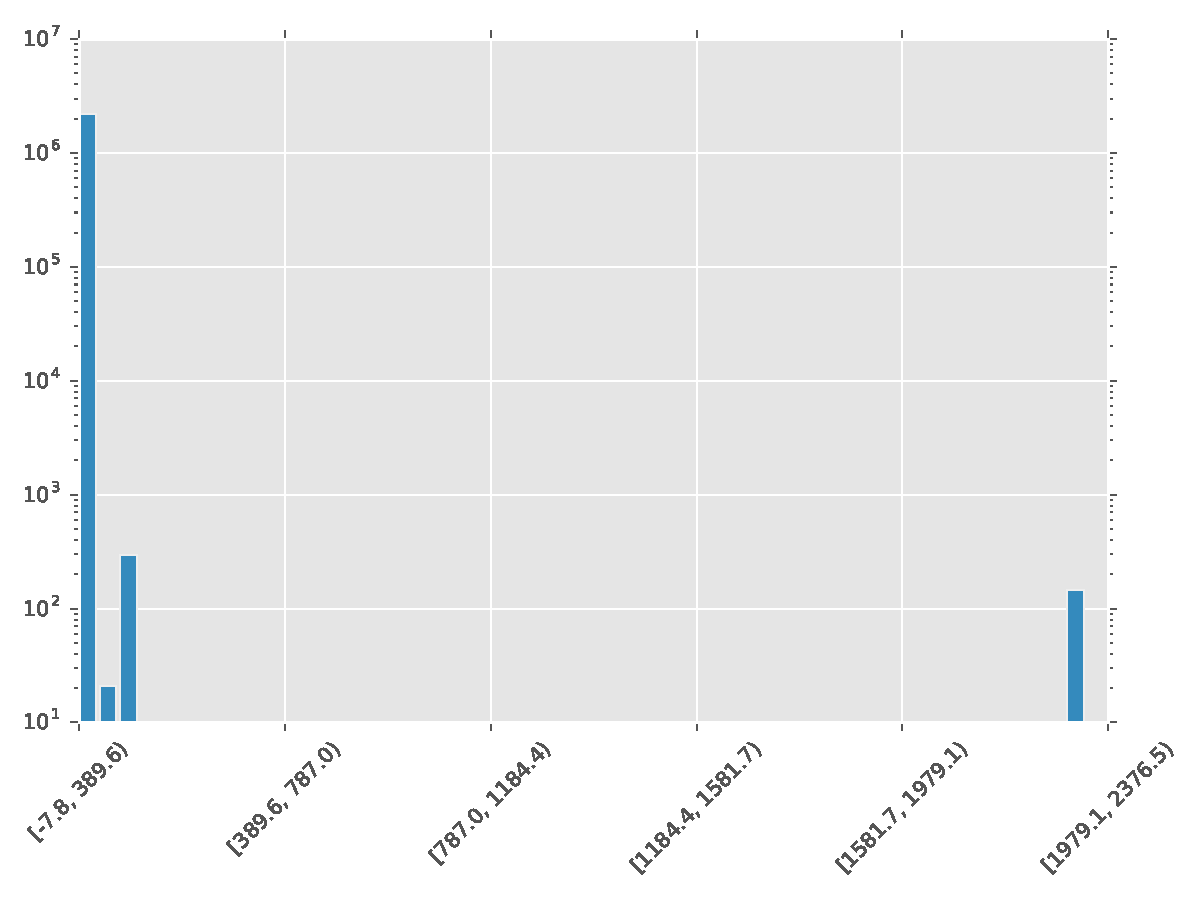
\includegraphics[width=\textwidth]{resources/histogramC}
        \caption{Histogram of weight values distribution.}
    \end{subfigure}%
    ~
    \begin{subfigure}[b]{0.32\textwidth}
        \centering
        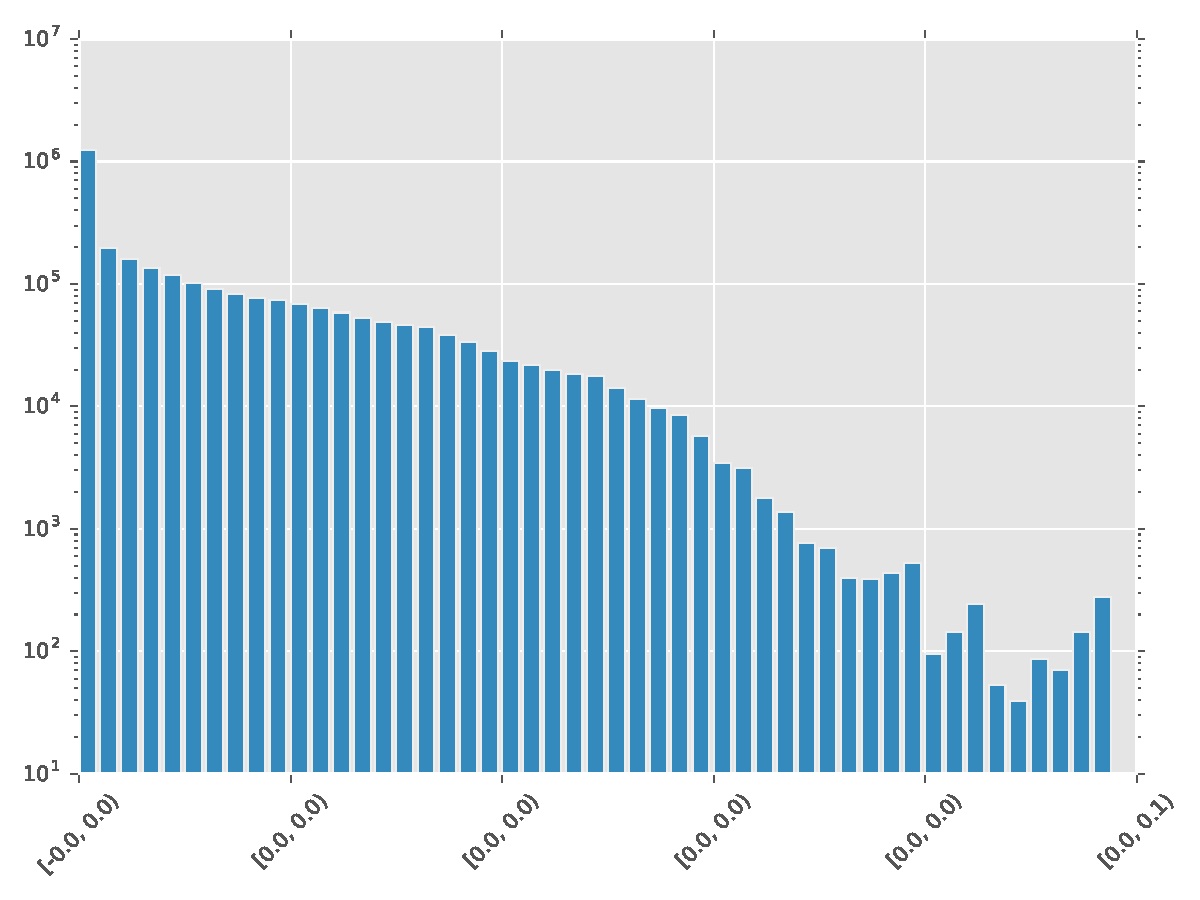
\includegraphics[width=\textwidth]{resources/histogramp}
        \caption{Histogram of pdf model values distribution.}
    \end{subfigure}
    ~
    \begin{subfigure}[b]{0.32\textwidth}
        \centering
        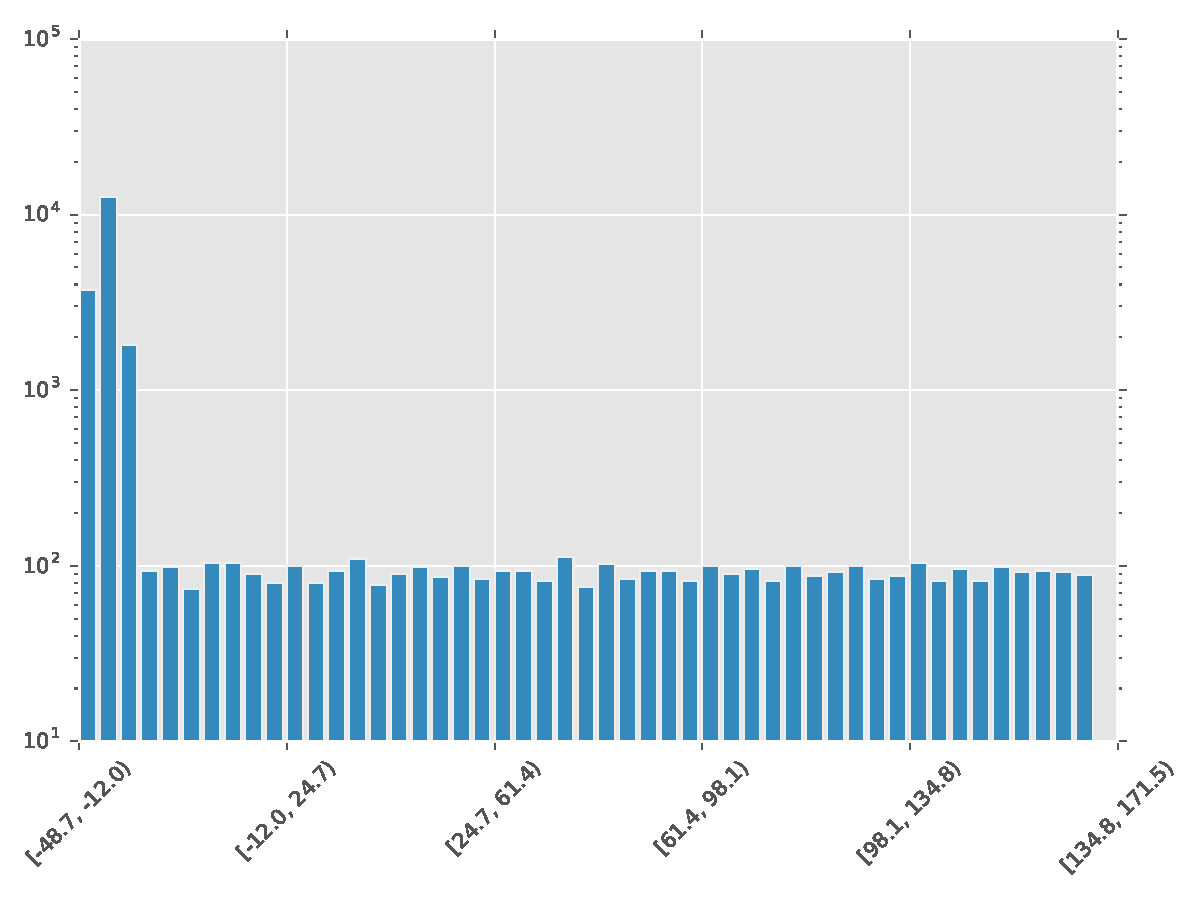
\includegraphics[width=\textwidth]{resources/histogramE}
        \caption{Histogram of E. kernel values distribution.}
    \end{subfigure}
    \caption{Value distributions}
    \label{fig:value-distributions}
\end{figure}


\begin{table}[H]
    \centering
    \caption{The final ranges}
    \label{tab:final-ranges}
    \begin{tabular}{lll}
        \toprule
        \textbf{Value set} & \textbf{Range Min} & \textbf{Range Max} \\
        \midrule
        Weight      &  \num{-2048}  &  \num{2048}     \\
        PDF model   &  \num{-1/8}   &  \num{1/8}      \\
        E. kernel      &  \num{-1/512} &  \num{1/512}    \\
        \bottomrule
    \end{tabular}
\end{table}

The speed-up that was measured with a fixed-point implementation based on the \texttt{int32\_t} type, and all values using the largest range (\num{2048}) was about \num{18} to \num{18.6} times kernel speed-up.
The problem is getting a faster conversion from the different ranges and a quick division that respects the fixed point nature of the values in the \texttt{int32\_t} datatype.
Instead of doing a normal integer division, although adding a shift to the nominator should give correct results.
To implement fixed-point math properly the project would need parts of boost for the operator overloads to create a good class, so all the errors and other debugging issues go away.
But linking boost just for that is a step too far for this project.
It was decided to drop the fixed point implementation.

After some benchmarking we found that a 4 way f32 mult takes about 9 cycles, a 4 way 32 mult takes about 5 cycles, and 8 way 16 bit mult takes 3 cycles.

\end{document}